\documentclass{article}
\usepackage{graphicx}
\begin{document}

\title{JOURNAL FOR LiDAR-VISION}
\author{Ayush Nayak}
\date{\today}

\maketitle

\begin{abstract}
    This is just the daily journal of my musings with this project, and where it will go. hanks!
\end{abstract}

\newpage

\section{June 25th}

This is the day that I started the journal, and started coding in the basic \LaTeX. The basic outline for the project, is to use LiDAR sensors to take in the surroundings, and then feed that into a computer, which determines all the obstacles, and then translates them into sound, which is played back through Dolby Atmos. The entire thing should be able to be compacted into a single pair of glasses, with a small LiDAR detector on top.

\section{June 29th}

The new Air Pods Pro feature is a must, where it has surround sound, as well as gyroscopes to show where everything is.

If I ever get serious about this, Airpods Pro + an iPhone XR and a LiDAR Helmet piece would probably be perfect. Dolby Atmos support is also pretty awesome, maybe WM300 XM3. Surround Sound + Lidar Detection, although I'm not super sure about how useful it would be to have lidar input, and how easy it is to differentiate different objects.

\section{June 30th}
So I am going to split this into two parts.

The first part is the actual LiDAR point detection and image classification, while the second type is the actual translating that LiDAR image into objects and classifying them. The second part is to actually take that plane of classified images, and turn it into audio signals through Dolby Atmos. 

Each day, I will just mark Part 1, and Part 2, and update each one individually. 

\textbf{Part 1:}

First, in order to detect whats going on, 3D and 2D classification will be used, preferably, through the KITTI dataset for 3d and 2d objects, through C++ for super fast execution, as this will have to happen on my terrible i7 5700xt for AI. Maybe use TensorFlow Lite C++ to train an embedded package. 
- I will have to build a camera detection system that can detect basically any object, using open source datasets, and then verify that object with the LiDAR Sensor, which may be more optional, although is more for distance than actual image classification. 

A diagram of the different classification and warning sites can be shown below.
\begin{figure}[htbp]
    \centerline{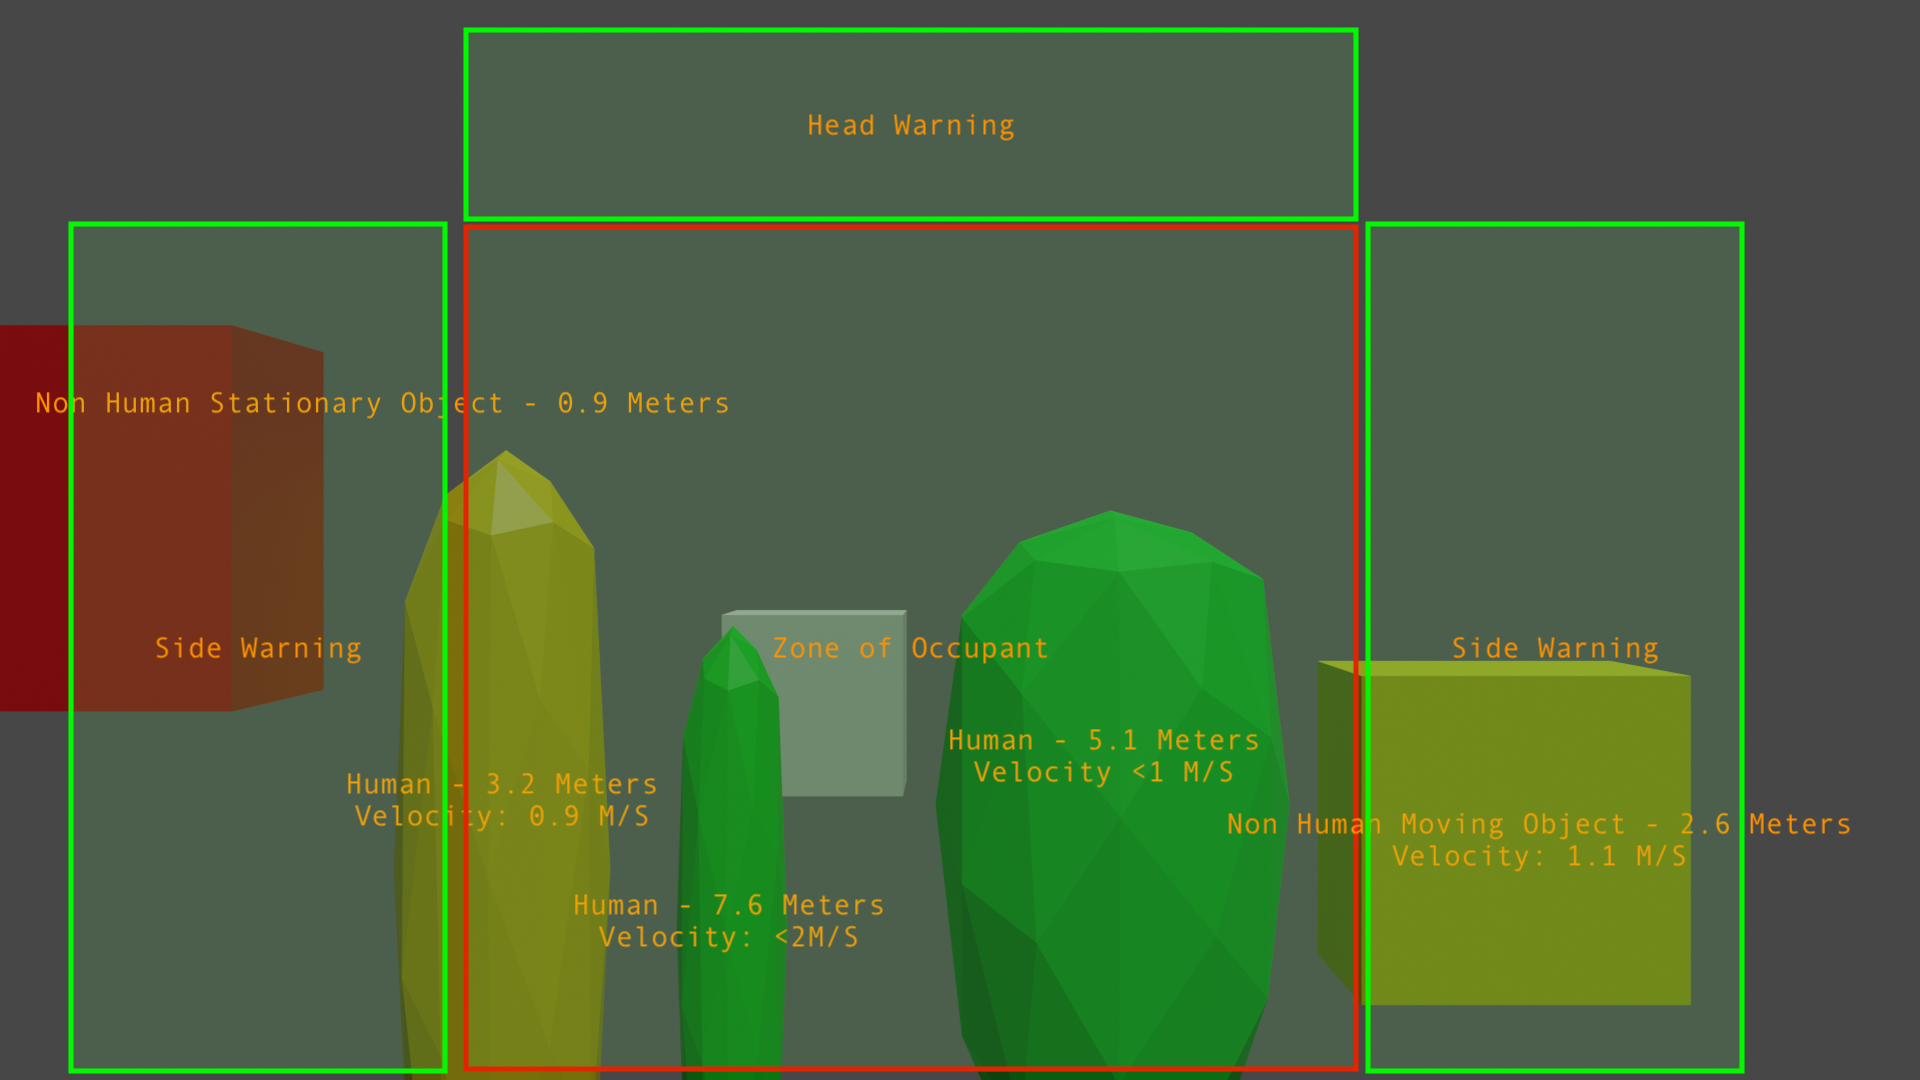
\includegraphics[scale=0.3]{Images/topviewtestsfrontview0.png}}
    \caption{This is a front view of classification space. At a basic level, things are classified as Humans, Cars, Stationary Objects, and Moving Objects. Different stages of warning are given.}
    \label{fig1}
\end{figure}

\begin{figure}[htbp]
    \centerline{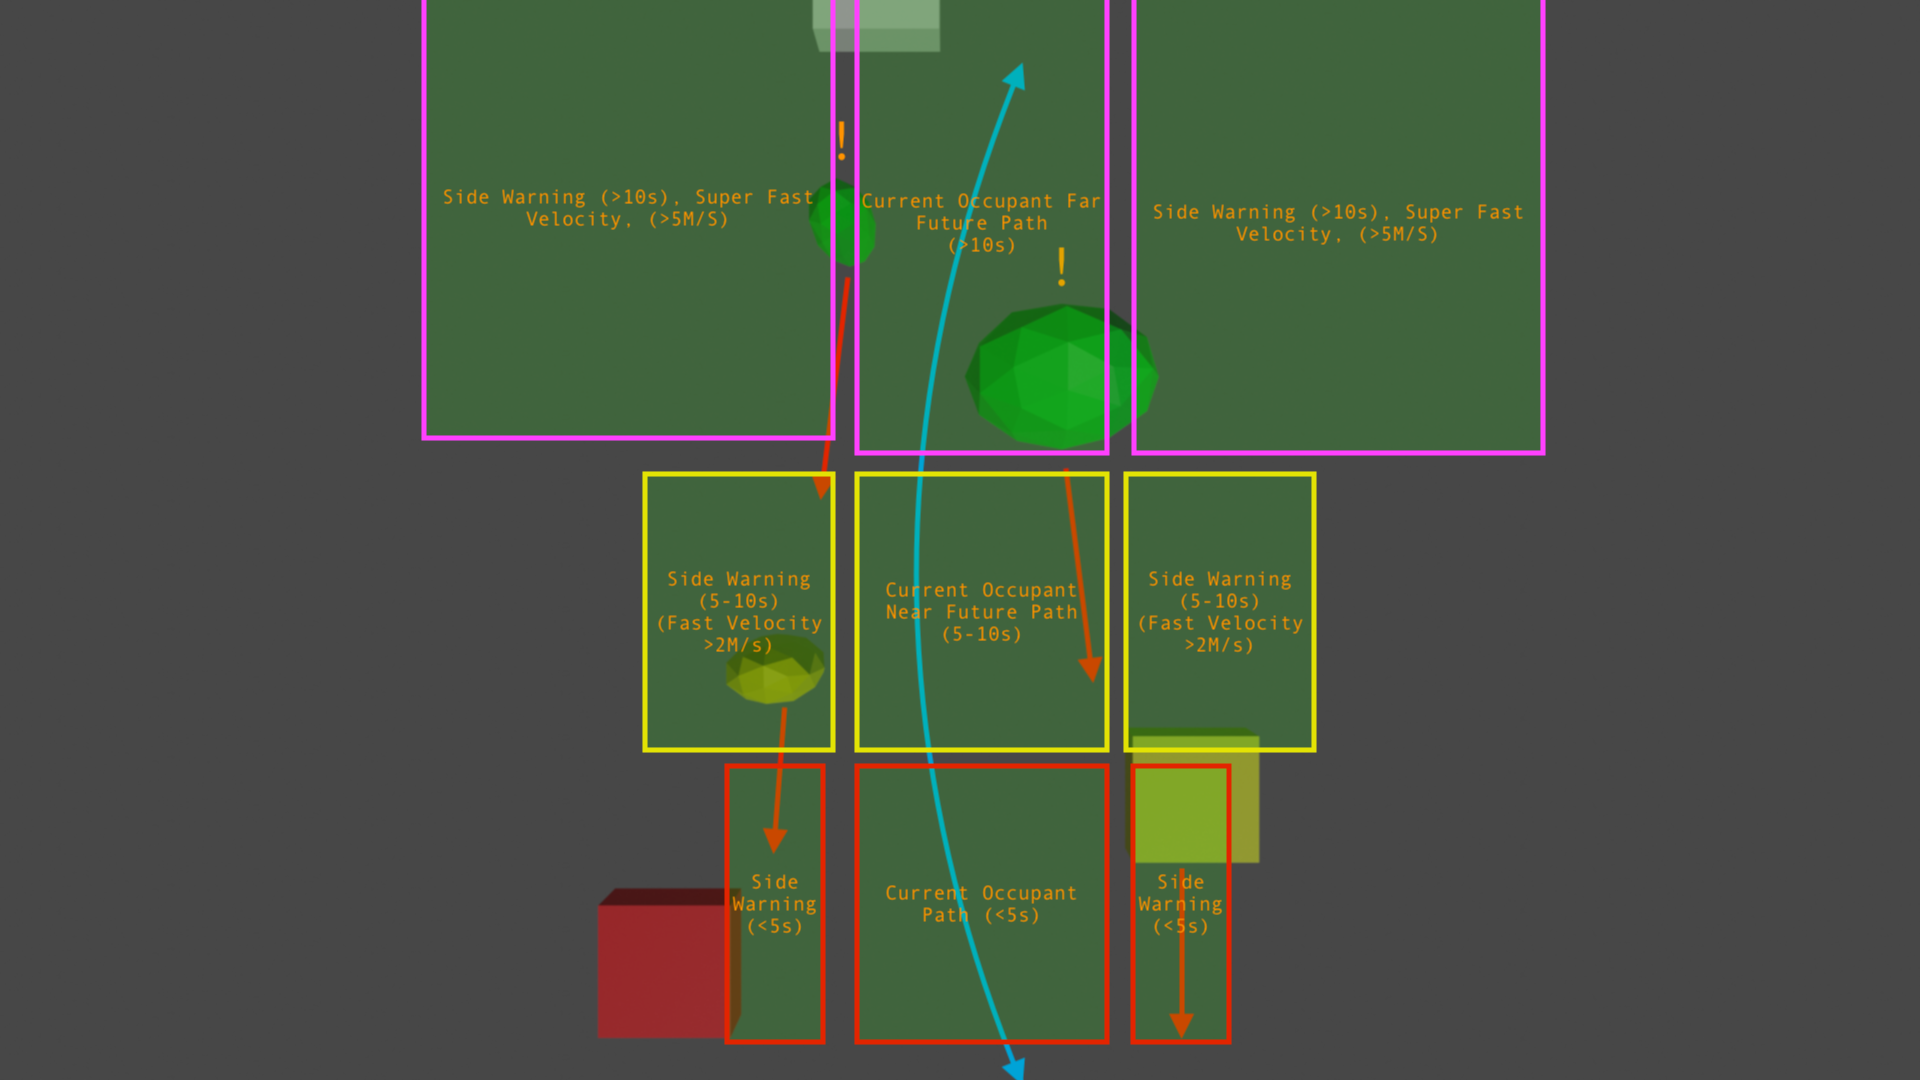
\includegraphics[scale=0.3]{Images/topviewtestset0.png}}
    \caption{This is a top view of classification space. At a basic level, things are classified as Humans, Cars, Stationary Objects, and Moving Objects. Different stages of warning are given, and here one can see why LiDAR is needed, as even for humans, it is very tricky to tell the distance of objects from the top perspective picture without labels}
    \label{fig2}
\end{figure}

For basic classification, a minimum amount of classes are needed, summarized in the table below

\begin{tabular}{ |p{2.5cm}||p{2.8cm}||p{1.8cm}||p{2.45cm}|  }
    \hline
    \multicolumn{4}{|c|}{Different categories for ultrabasic image classification } \\
    \hline
    Moving & Ground Changes & Stationary & Humans\\
    \hline
    \hline
    Cars            & Slope             & Pole      & Stationary\\
    Bikes           & Large Bump        & Booth     & Medium Fast\\
    Wheeled Object  & Small Bump        & Store     & Drunk/Random\\
    Large Pushcart  & Dropped Obstacle  & Hydrant   & Signaling\\
    Scooter         & Fluid             & Zoned Area& \\
    Animal          & Texture Change    & Door      & \\
    Other Moving    & Place to Stop     &           & \\
                    & Other             &           & \\
    \hline
\end{tabular}

    
Classification for these objects will be in two ways, first of all, if they are moving, velocity, and expected path, and how it conflicts with the current movers path, this can be seen in the second image. Secondly, identifying the type of change, whether it is in range, and then accordingly warning the occupant.

\section{July 1st}

\textbf{Part 1:}

Training the AI to recognize the background, through a combination of LiDAR and visible imagery, the LiDAR to categorize into Moving, Ground and Stationary, and the visible to further classify the different parts into their constituent parts, as well as train the computer to recognize combined LiDAR and visible images. The small list of objects that has been lain out to work should be enough, to provide comprehensive enough information. For off-sidewalk style walking, as well as GPS navigation to certain places, gyroscopes and the visible light system can be used for Google Maps API integration, while the LiDAR + Visible is used to warn about obstacles. In terms of changing ground, this is more for slippery obstacles or unseen objects in the path of one's feet than actual ground changes. For instance a step down into terrain would be a warning, while asphalt to cement if there is no serious incline would not. A serious incline would be about 10cm. LiDAR has to be aimed to record the ground and "ceiling" to record sufficient information.

The detection would be split into 3 ways. The omnipresent object detection and warning, which warns about obstacles, and other humans. Meanwhile, one can choose between navigation, and just general detection. Navigation would utilize the Google Maps API to route people through sidewalks and crosswalks, to their destination, while a more free roam general detection would let them search around and would highlight all the different obstacles. This combination will help people to get where they are going.

\textbf{Part 2}

I didn't do Part 2 for yesterday, but honestly other than trying to think of a way to make different noises, its pretty basic for now. 

All four different stages will have their own feel and look

\end{document}